% Chapter Template

\chapter{ANN Algorithm} % Main chapter title

\label{Chapitre 3} % Change X to a consecutive number; for referencing this chapter elsewhere, use \ref{ChapterX}

\lhead{ \emph{Using ANN for gesture recognition}} % Change X to a consecutive number; this is for the header on each page - perhaps a shortened title

%----------------------------------------------------------------------------------------
%	SECTION 1
%----------------------------------------------------------------------------------------
\section{Project inspiration}
Avant de se lancer tête baissée sur le projet, il faut prendre le temps de réfléchir et de s'inspirer d'autres projets effectués. Nous avons consulté quelques papier intéressant, notemment sur les "features" utilisée dans un système de reconnaissances de geste, afin de tirer les élément interressant pour notre système.

Voici les quelques traités principale qui nous ont aidés dans cette recherche :

\begin{itemize}
\item Utiliation de la transformée en ondelette dans un système de classification ANN pour détecter des problèmes coronariens(Lund University) \footnote{http://lup.lub.lu.se/luur/download?func=downloadFile\&recordOId=2204713\&fileOId=2204714}
\item Reconnaissance de geste grâce à une accéléromètre et un système de classification ANN (Instituto Panamericano de Investigación Tecnológica)
\footnote{ http://www.researchgate.net/profile/Carlos\_Delgado-Mata/publication/257743699\_ANN\_for\_Gesture\_Recognition\_using\_Accelerometer\_Data/links/0deec52d2853a37172000000.pdf}
\item Reconnaissance de geste avec les signaux "EMG"(Karunya University) \footnote{http://www.rspublication.com/ijca/ijca\_index.htm}
\item Et le plus intéressant "Analysis and Selection of Features for Gesture Recognition Based on a Micro Wearable Device" (University of Aizu) \footnote{http://citeseerx.ist.psu.edu/viewdoc/download?doi=10.1.1.220.2560\&rep=rep1\&type=pdf}
\end{itemize}


\section{Physical data choices}
En nous basant sur la dernière de ces documentation, nous avons remarqué que le centre de la reconnaissance ne se trouve pas dans l'utilisation d'un grand nombre de grandeur physique et de capteurs, mais dans l'extraction des bonnes caractéristique d'un signal temporel.\\

Evidemment, le choix du capteur est tout de même important. Il faut choisir un capteur qui est le plus représentatif de tout les gestes. Par exemple, le capteur de l'épaule n'est absolument pas représentatif du système.
Nous avons choisi le capteur de la main uniquement. C'est le capteur qui possède le plus d'informations intéresssantes pour la pluspart (voir la totalité) des gestes. Nous avons testé le système avec plusieurs capteurs, mais les résulats obtenus n'ont montrés aucune améliorations, voir même de légeres dégradations.\\

Reste maintenant le choix des grandeurs physique. Le capteur est une chose, mais il faut aussi choisir les grandeurs physique les plus représentative. Ce qui nous intéressait, c'était de connaître les différentes inclinaisons de la main en fonction du temps et de la position (magnitude) de celle-ci. Pour cela nous avons choisi les grandeurs suivante :
\begin{itemize}
\item Yaw,Pitch et Roll (inclinaisons)
\item Magnitude X,Y et Z (Magnitude du déplacement)

\end{itemize}

\pagebreak
\section{Signal features extraction}
Nous arrivons maintenant à la partie clé de ce projet : l'extraction de données intéressante du signal. En nous basant sur les différentes observation et résulats des publications que nous avons lues, nous avons essayés différentes features possible.\\

Nous avons commencé par effectuer un pré-traitement des signaux, histoire d'enlever un maximum de bruit à ceux-ci. Pour cela, nous avons utilisé un filtre passe-bas qui déphase peu le signal (Nous ne voulons pas perdre d'informations). Voici ci-dessous la résponse en "fréquence" de notre filtre :

\begin{center} 
\hspace{15cm}
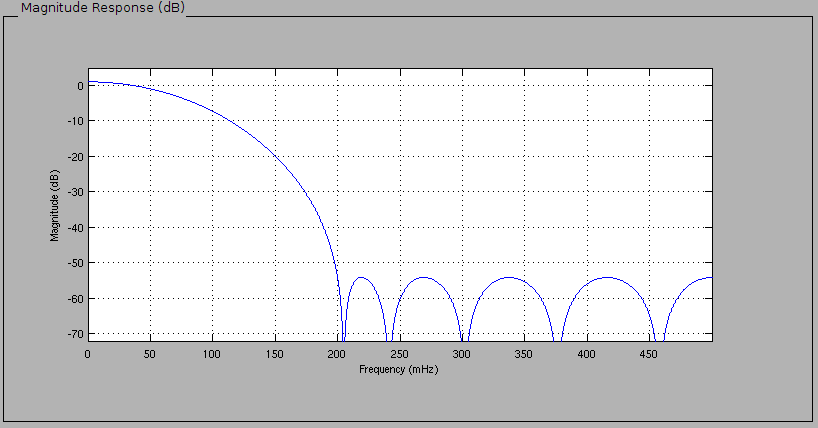
\includegraphics[width=15cm]{Filter.png}
\end{center}
\vspace{0.5cm} 

Une fois les signaux filtrés, on peut essayer de fusionés un couple X,Y,Z en un seul signal en l'additionnant (que l'on va appeler signal fusionné). Donc si on utilise deux grandeur physique, on aura 2 couples X,Y,Z et donc 2 signaux fusionnés. \\

De plus, nous dérivons aussi les signaux X,Y et Z, ce qui nous donnes aussi une très bonne information sur la rapidité de transition de ceux-ci. Par exemple, le mouvement de calibration bouge très peu par rapport au mouvement "bonjour" de la main. 

\pagebreak 
Voici une représentation tempporelle et fréquenciel du mouvement "Shake" :

\begin{center} 
\hspace{15cm}
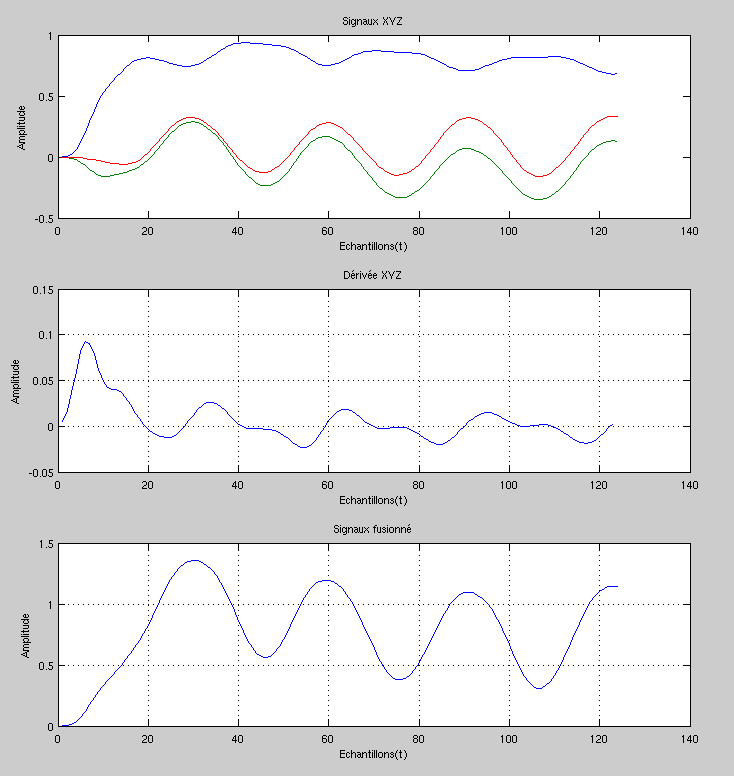
\includegraphics[width=15cm]{Hand11_amp_sig.png}
\end{center}
\vspace{0.5cm} 

\begin{center} 
\hspace{15cm}
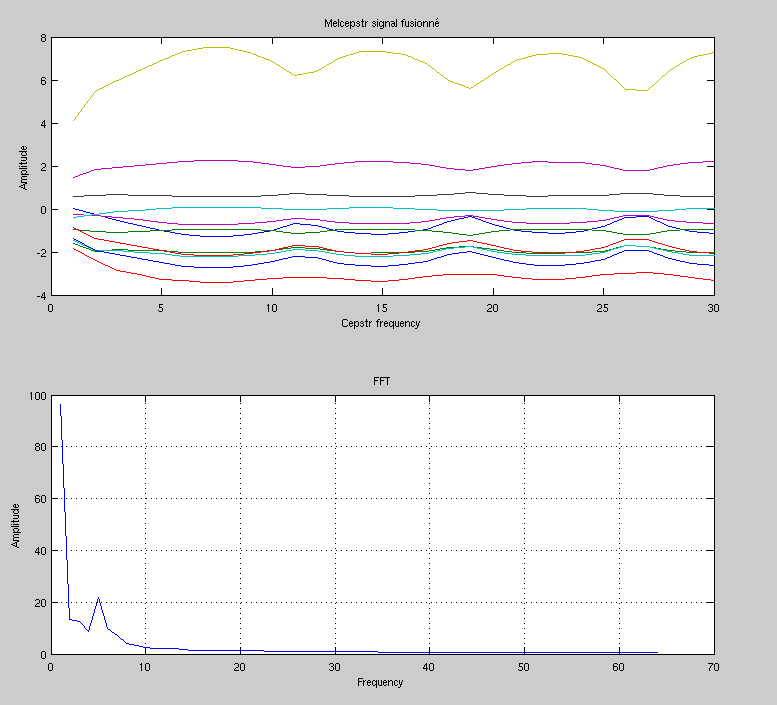
\includegraphics[width=15cm]{Hand11_amp_melcepstr.png}
\end{center}
\vspace{0.5cm} 

On peut bien observer sur le graphique de la FFT, la composante continue et le pique de fréquence généré par le mouvement. Ceci dit, nous avons trouvé une features excentrique, qui à considérablement poussé les résultats de notre système : les "melcepstres". Initialement utilisés pour extraire les données de la voix, nous avons pensé de les tester sur notre signal fusionné (c'est aussi un signal temporel. Voir chapitre sur les résultats).\\

Comme dit précédement, il faut extraire maintenant les données des différents signaux ( X,Y,Z, signal fusionné et les différentes dérivées). Ce qu'il ne faut pas oublier, c'est que les réseaux de neurones ne peuvent pas prendre les signaux temporels directement en entrée. Voici les features utilisées, basés sur l'étude des différentes publiation :
\begin{itemize}
\item[\textbf{Sur les signaux X,Y,Z :}]
\item Valeur moyenne : utilisée de bases, mais n'est que très peu représentative des gestes.
\item L'écart-type : c'est une très bonne features couplée à la valeur moyenne.
\item L'énergie du signal : nous ne pouvons pas bien quantifier son effet sur le système. Mais elle apporte tout de même des meilleurs scores.
\item Valeur "peak-peak" : c'est une excellente feature, car elle apporte une bonne information sur l'amplitudes des mouvements.
\item Dynamic Time Warping : Nous avons essayé de correler différents axes entre-eux, mais sans grand succès sur les performances. Toutefois, ce serait une chose à reconsidérer avec le système actuel.\pagebreak

\item[\textbf{Sur les signaux X',Y',Z' :}]
\item Valeur moyenne : Très utile, car elle démontre directement la rapidité ou la périodicité d'un mouvement.
\item L'énergie du signal : nous ne pouvons pas bien quantifier son effet sur le système. Mais elle apporte tout de même des meilleurs scores.\\

\item[\textbf{Sur les signaux fusionnés (+ fusionnés dérivés):}]
\item Nombre de peaks : améliore un peu les scores.
\item "Melcepstres" (valeur moyenne, écart-type et énéregie sur ceux-ci) : il amènent un excellent score. 

\item[\textbf{Sur la FFT des signaux fusionnés:}]
\item On utilise directement la représentation fréquencielle de celle-ci. Cela signifie 64 échantillons (ou 64 entrée ANN supplémentaires)
\end{itemize}

\section{ANN implementation}

Voici une simple illustration de notre réseau :
\begin{center} 
\hspace{15cm}
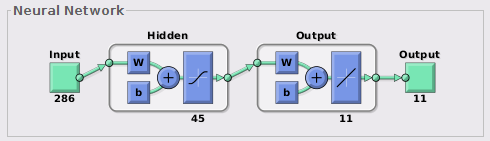
\includegraphics[width=15cm]{NetView.png}
\end{center}
\vspace{0.5cm} 

Nous avons mesurés les performances avec la méthode "Mean Squared Error" et nous avons entrainés le système avec l'algorithme "Levenberg-Marquardt" (nous avons aussi essayé «Scaled Conjugate Gradient», mais celui-ci ne convergait pas pour notre système).\\

Nous avons découper notre "dataset" en trois parties :
\begin{itemize}
\item Training = 70\%
\item Validation = 15\%
\item Test = 15\%\\

\end{itemize}

Nous n'avons malheureusement pas implémenter de "cross-validation" (le temps étant court). 

\pagebreak
\section{Performance and results}

Voici les performance mesurées de notre système ANN (MSE):
\begin{center} 
\hspace{15cm}
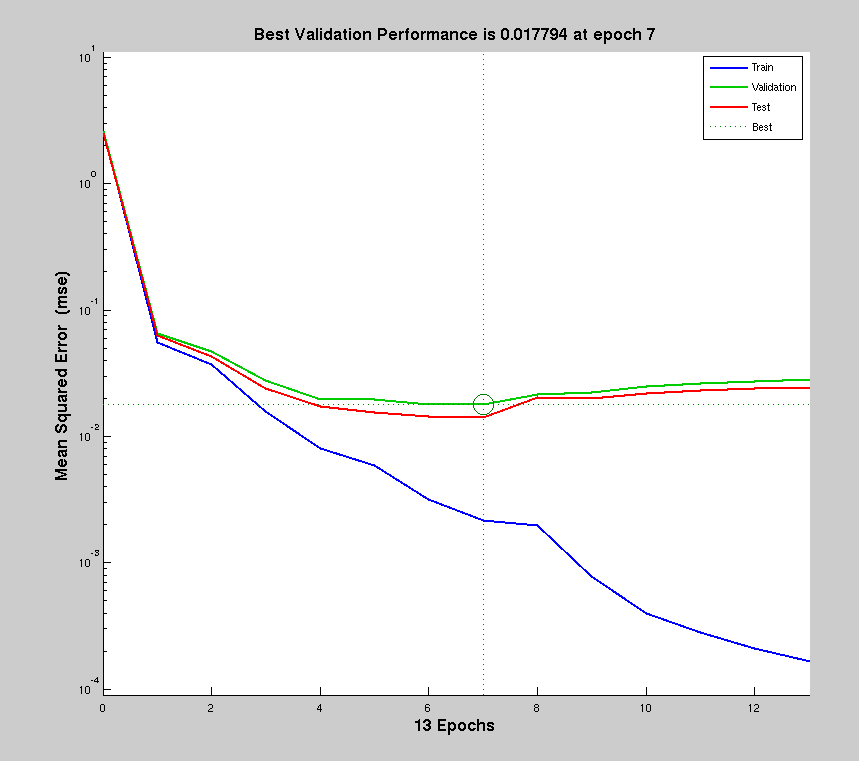
\includegraphics[width=15cm]{MsePlot.png}
\end{center}
\vspace{0.5cm} 

Il nous faut faire attention à ne plus rajouter trop de features, car le système commence à être en situation de "overfitting" et commence à aprendre notre "dataset" par coeur.\\


Au début, nous obtenions des résultat de l'ordre de 50\%. Mais après l'introduction des "melcepstres" et l'augmentation des la taille de la couche cachée, le score est passé à 96\% !\\

Et en ajoutant encore la FFT, le score et passé à 99,3\%. Ce qui est assez impressionant. Voici la matrice de confusion, qui nous montre la répartition des erreurs sur notre système:
\begin{center} 
\hspace{15cm}
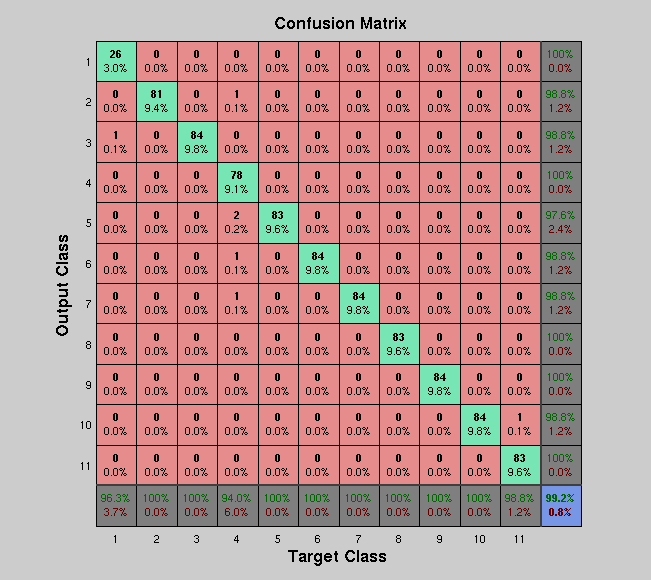
\includegraphics[width=15cm]{ConfusionMatrix.png}
\end{center}
\vspace{0.5cm} 

On remarque qu'il existe encore des problème entre les mouvement "take from screen" et "push to screen". 

\section{Possible improvement}

Notre système était basé sur le score plutôt que les performances. On pourrait par exemple réfléchir quels features sont inutiles, ou pas indipensable. \\

Pour améliorer notre score, on pourrait implémenter une "cross-validation" pour notre système. Voir même essayer d'ajouter le DTW comme features sur notre système (attentions toutefois aux performances !)
